Som nævnt i afsnit \ref{sec:valgafvaektoej}, bliver dette projekt udviklet agilt. Et af kendetegnene ved agile udviklingsmetoder er at 
planlægning foregår undervejs i forløbet i modsætning til for eksempel vandfaldsmetoden, hvor planlægning er en 
forudsætning for arbejdets påbegyndelse. På baggrund af dette, findes det relevant at bruge tid på at diskutere 
risikohåndtering. Risikohåndtering består af 4 punkter:

\begin{itemize}
    \item Identifikation af risici
    \item Tildeling af sandsynlighed
    \item Evaluering af konsekvenser
    \item Hvordan skal risici håndteres?
\end{itemize}

Formålet med dette kapitel er at diskutere disse 4 punkter, og redegøre for hvordan gruppen har håndteret risikoanalyse/håndtering. \\ 

Som noget af det første i projektperioden, har gruppen forsøgt at identificere en række af ting som kan have negativ indflydelse
på tidsplanen, skulle de indtræffe. Gruppen har her forsøgt at forholde sig til risici, som anses for at være forholdvis realistiske, for ikke
at ende med et risk register der er alt for omfattende. Gruppen har identificeret risici inden for de følgende områder:

\begin{itemize}
    \item Fravær
    \item Konflikthåndtering
    \item Planlægning
    \item Projektkrav
\end{itemize}

I Figur \ref{fig:riskregister} kan gruppens risk register ses. Et risk register viser de risici gruppen har identificeret, samt gruppens vurdering af, hvor sandsynligt det er, at de indtræffer.

\begin{figure}[H]
    \centering
    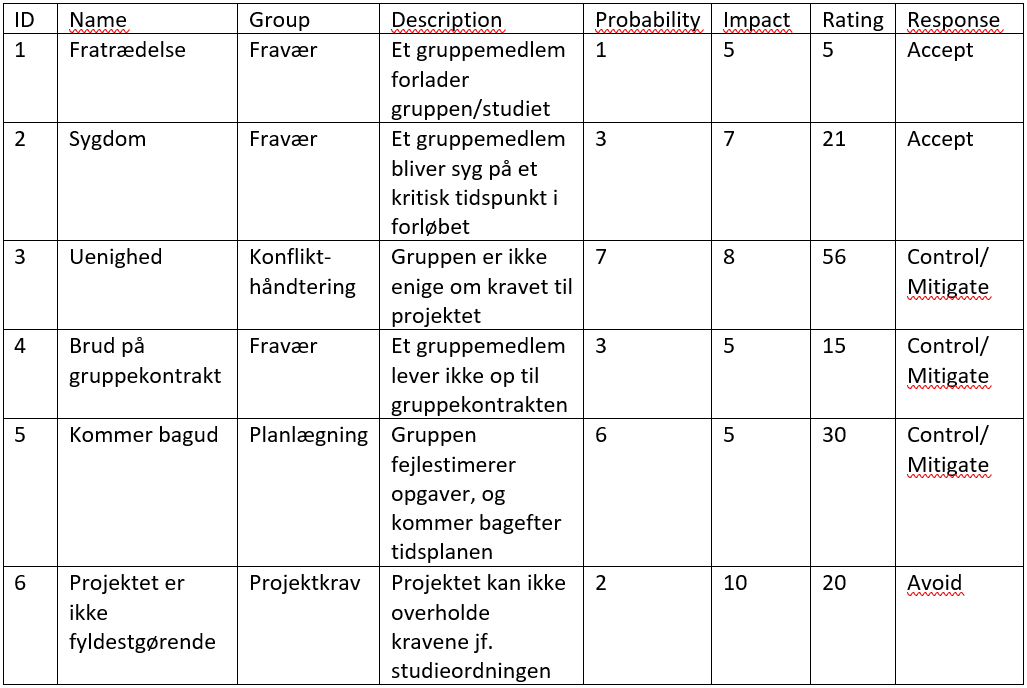
\includegraphics[width=\textwidth]{figures/RiskRegister.png}
    \caption{Risk register}
    \label{fig:riskregister}
\end{figure}

Som det fremgår i figuren, har hver risiko fået en respons: Accept, Control/Mitigate, eller Avoid. De risici, der har fået responsen accept, vil gruppen ikke gøre
noget særligt ud af, da dette kan være besværligt ved ting som for eksempel sygdom. De risici der har fået responsen control/mitigate, vil gruppen forsøge at forhindre,
inden problemet indtræffer. Risici med responsen avoid, vil projketgruppen gøre alt hvad der er muligt for at forhindre til enhver tid. \\

I Figur \ref{fig:riskmanagement} ses en tabel der beskriver hvordan gruppen vil håndtere de risici der enten har responsen control/mitigate eller avoid.

\begin{figure}[H]
    \centering
    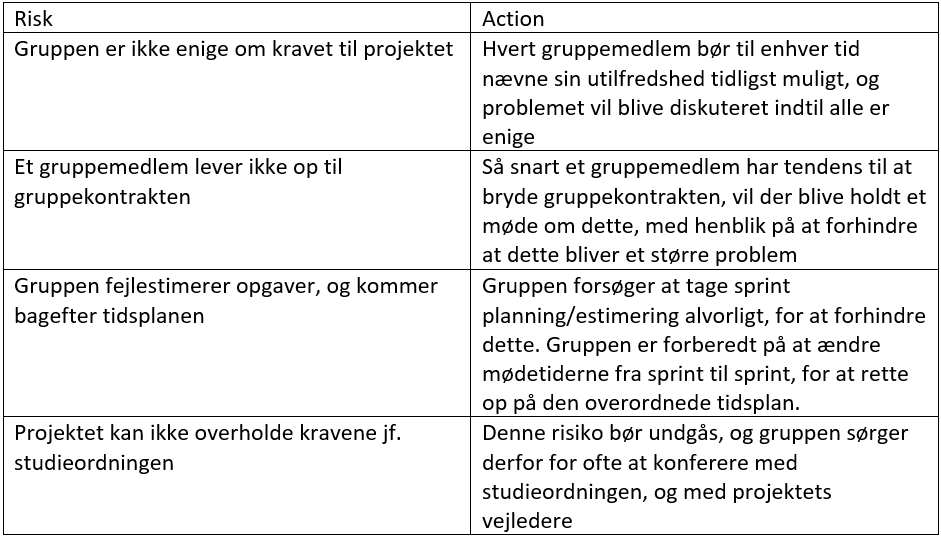
\includegraphics[width=0.7\textwidth]{figures/RiskAction.png}
    \caption{Håndtering af risici}
    \label{fig:riskmanagement}
\end{figure}